\chapter{Schwartz}

\section{15: The Casimir effect}

\subsection{Main idea}
This chapter showed two important things using the example of a field in a box:
\begin{itemize}
    \item UV divergence i.e. infinite contribution due to the contribution from arbitrarily small frequencies can be dealt by placing a lower cutoff.
    \item During the intermediate calculations we need to work in a finite sized box and at the end we can take the outer box to be of infinite size. This is to avoid getting infinite contributions during the calculations and will not affect the final force. We can avoid this box by using counterterms which are themselves infinite but drop of when we finally calculate anything physical.
\end{itemize}

\begin{itemize}
    \item Casimir force is independent of any regulator as long as 
    \begin{equation}
        \lim _{x \rightarrow \infty} x f^{(j)}(x)=0 \quad \text { and } \quad f(0)=1
    \end{equation}
    \item It is an infrared effect
\end{itemize}

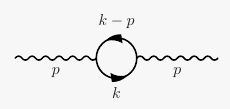
\includegraphics{chapters/QFT/images/image1.png}
